\newpage
% ============================================================
\section{Actividad 2: Evaluación con Secuencias LRD}
% ============================================================

Se evalúan los estimadores \texttt{vt2} y \texttt{LD2} sobre secuencias
sintéticas con dependencia de rango largo (LRD), generadas con \texttt{betamwm}
(multifractal) y \texttt{wfbm} (monofractal), para
$H \in \{0.55,\, 0.60,\, \dots,\, 0.95\}$ con $1\,000$ repeticiones por
valor de $H$. Las propiedades evaluadas son sesgo, eficiencia y consistencia.

% ------------------------------------------------------------
\subsection{Prueba de Sesgo}
% ------------------------------------------------------------

Para construir la Figura~\ref{fig:sesgo_a2} se realizó un sondeo sistemático
del sesgo por cada valor de $H \in \{0.55,\, 0.60,\, \dots,\, 0.95\}$
(incrementos de $0.05$, nueve puntos en total) se generaron $1\,000$
realizaciones independientes con cada generador y se aplicaron los estimadores
\texttt{vt2} y \texttt{LD2}. El valor medio $\hat{\mu}$ de las $1\,000$
estimaciones se tomó como representante del estimador en ese punto y se
graficó contra $H$ real. La diagonal punteada representa el estimador ideal
$\hat{H} = H$; la distancia vertical entre cada curva y la diagonal es el
sesgo empírico $\hat{\mu} - H$ para ese valor de $H$.

\begin{figure}[H]
    \centering
    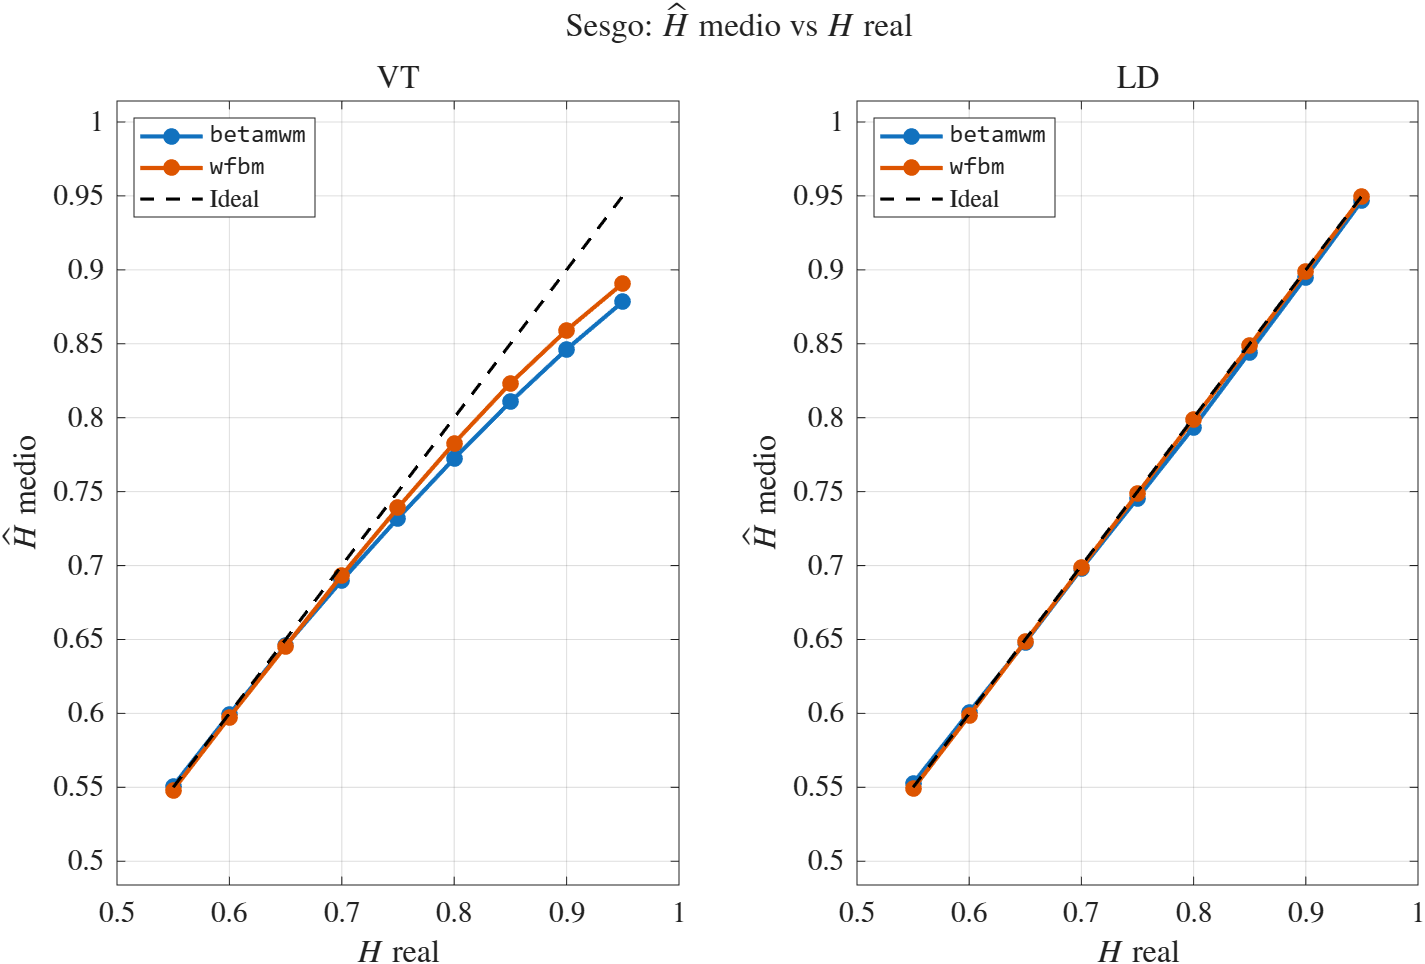
\includegraphics[width=0.95\textwidth]{actividades/actividad2/imgs/sesgo_vt_ld.png}
    \caption{Sesgo de los estimadores VT y LD para \texttt{betamwm} y
             \texttt{wfbm} ($1\,000$ repeticiones por valor de $H$).}
    \label{fig:sesgo_a2}
\end{figure}

\textbf{Estimador VT.} Ambos generadores producen subestimación creciente
con $H$. Para \texttt{betamwm}, el sesgo pasa de $-0.0023$ en $H = 0.55$
hasta $-0.0711$ en $H = 0.95$; para \texttt{wfbm}, de $-0.0016$ a $-0.0092$.
VT es considerablemente más sesgado con \texttt{betamwm} que con \texttt{wfbm}
para valores altos de $H$, lo que evidencia su sensibilidad a la naturaleza
multifractal del proceso.

\textbf{Estimador LD.} Las curvas se superponen casi perfectamente con la
diagonal ideal en ambos generadores. El sesgo máximo es $-0.0054$ para
\texttt{betamwm} ($H = 0.90$) y $-0.0010$ para \texttt{wfbm} ($H = 0.95$),
valores despreciables en todo el rango. LD estima $H$ con alta fidelidad
independientemente del generador y del valor de $H$.

\begin{table}[H]
\centering
\caption{Parámetros de ajuste normal y sesgo para el caso representativo
         $H = 0.9$ ($1\,000$ repeticiones).}
\label{tab:sesgo_a2}
\renewcommand{\arraystretch}{1.3}
\begin{tabular}{llccc}
\toprule
\textbf{Generador} & \textbf{Estimador} & $\hat{\mu}$ & $\hat{\sigma}$ &
\textbf{Sesgo} \\
\midrule
\texttt{betamwm} & VT & $0.8463$ & $0.0207$ & $-0.0537$ \\
\texttt{wfbm}    & VT & $0.8592$ & $0.0188$ & $-0.0408$ \\
\texttt{betamwm} & LD & $0.8951$ & $0.0377$ & $-0.0049$ \\
\texttt{wfbm}    & LD & $0.8989$ & $0.0143$ & $-0.0011$ \\
\bottomrule
\end{tabular}
\end{table}

La Figura~\ref{fig:qqplots_a2} presenta los QQ-plots de las
$1\,000$ estimaciones para $H = 0.9$ en las cuatro combinaciones
generadas frente al estimador.

\begin{figure}[H]
    \centering
    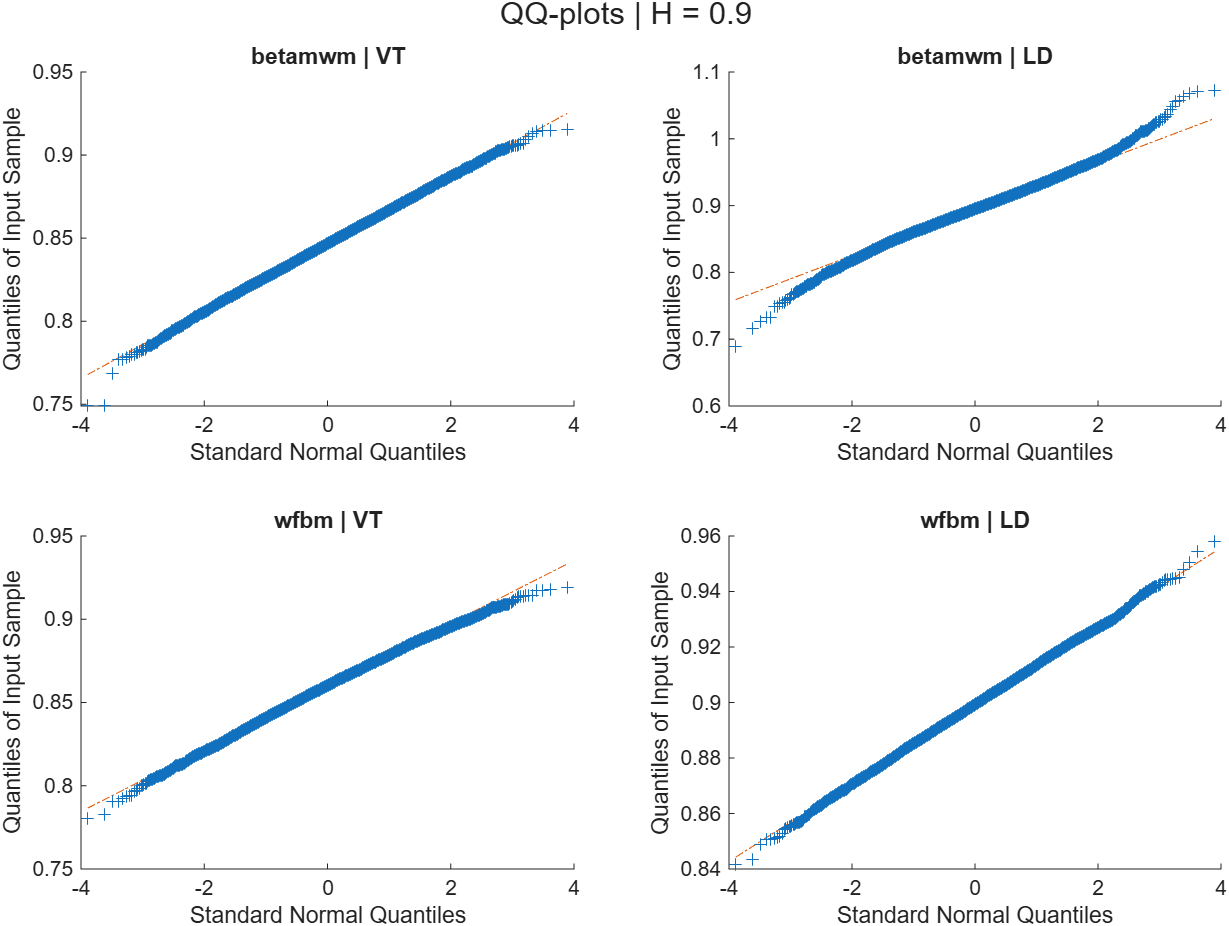
\includegraphics[width=0.95\textwidth]{actividades/actividad2/imgs/qqplots.png}
    \caption{QQ-plots de $\hat{H}$ para $H = 0.9$ ($1\,000$ repeticiones).}
    \label{fig:qqplots_a2}
\end{figure}

La imagen anterior confirma que las distribuciones empíricas de $\hat{H}$
siguen aproximadamente una normal.
Se observan diferencias cualitativas coherentes con el análisis de sesgo:

\begin{table}[H]
\centering
\caption{Resumen comparativo de ajuste, sesgo y dispersión para VT y LD sobre procesos multifractales y monofractales.}
\label{tab:qqplot_comparison}
\renewcommand{\arraystretch}{1.4}
\begin{tabular}{|p{3cm}|p{5.8cm}|p{5.8cm}|}
\hline
\textbf{Proceso} & \textbf{VT} & \textbf{LD} \\
\hline

\textbf{\texttt{betamwm}} 
&
Buen ajuste en el cuerpo central con leve desviación en la cola inferior.  
Distribución centrada en $\hat{\mu}=0.846$, alejada de $H=0.9$, consistente con un sesgo de $-0.054$.
&
Mayor dispersión de los cuatro casos ($\hat{\sigma}=0.038$), con desviación en ambas colas.  
La distribución permanece centrada cerca de $H=0.9$ (sesgo de $-0.005$), indicando mejor exactitud aunque con mayor varianza.
\\
\hline

\textbf{\texttt{wfbm}}
&
Buen ajuste con leve desviación en la cola superior.  
Distribución centrada en $\hat{\mu}=0.859$, con sesgo de $-0.041$, menor que en \texttt{betamwm} pero aún apreciable.
&
El ajuste más fiel a la recta de referencia, con la menor dispersión ($\hat{\sigma}=0.014$) y el menor sesgo ($-0.001$).  
Confirma que LD sobre secuencias monofractales representa el escenario más favorable.
\\
\hline

\end{tabular}
\end{table}

Las Figuras~\ref{fig:vt_h09} y~\ref{fig:ld_h09} muestran las PDF y CDF
empíricas para $H = 0.9$.

\begin{figure}[H]
    \centering

    \begin{minipage}{0.48\textwidth}
        \centering
        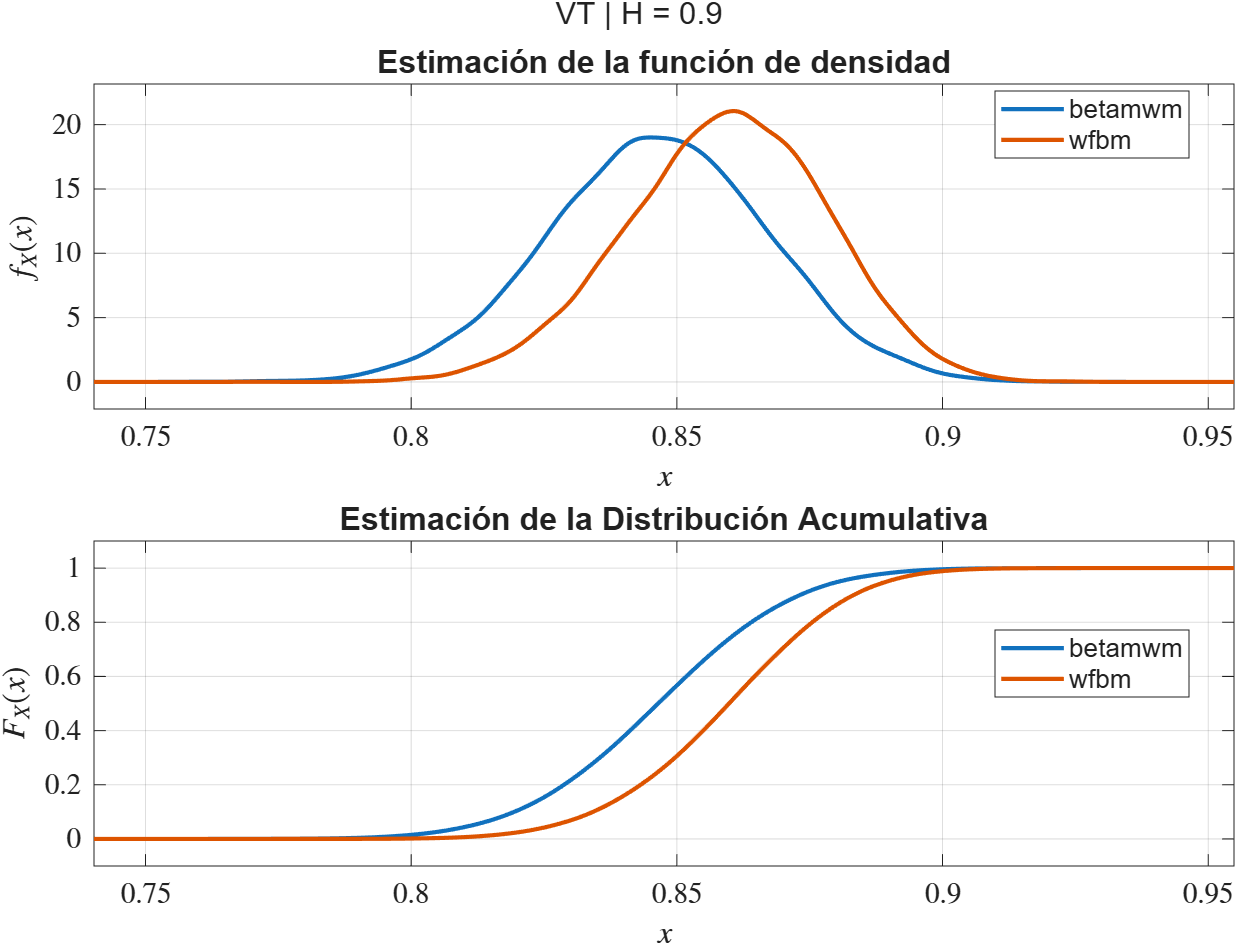
\includegraphics[width=\textwidth]{actividades/actividad2/imgs/VT_H0_9.png}
        \caption{PDF y CDF de $\hat{H}$ con VT para $H=0.9$.}
        \label{fig:vt_h09}
    \end{minipage}
    \hfill
    \begin{minipage}{0.48\textwidth}
        \centering
        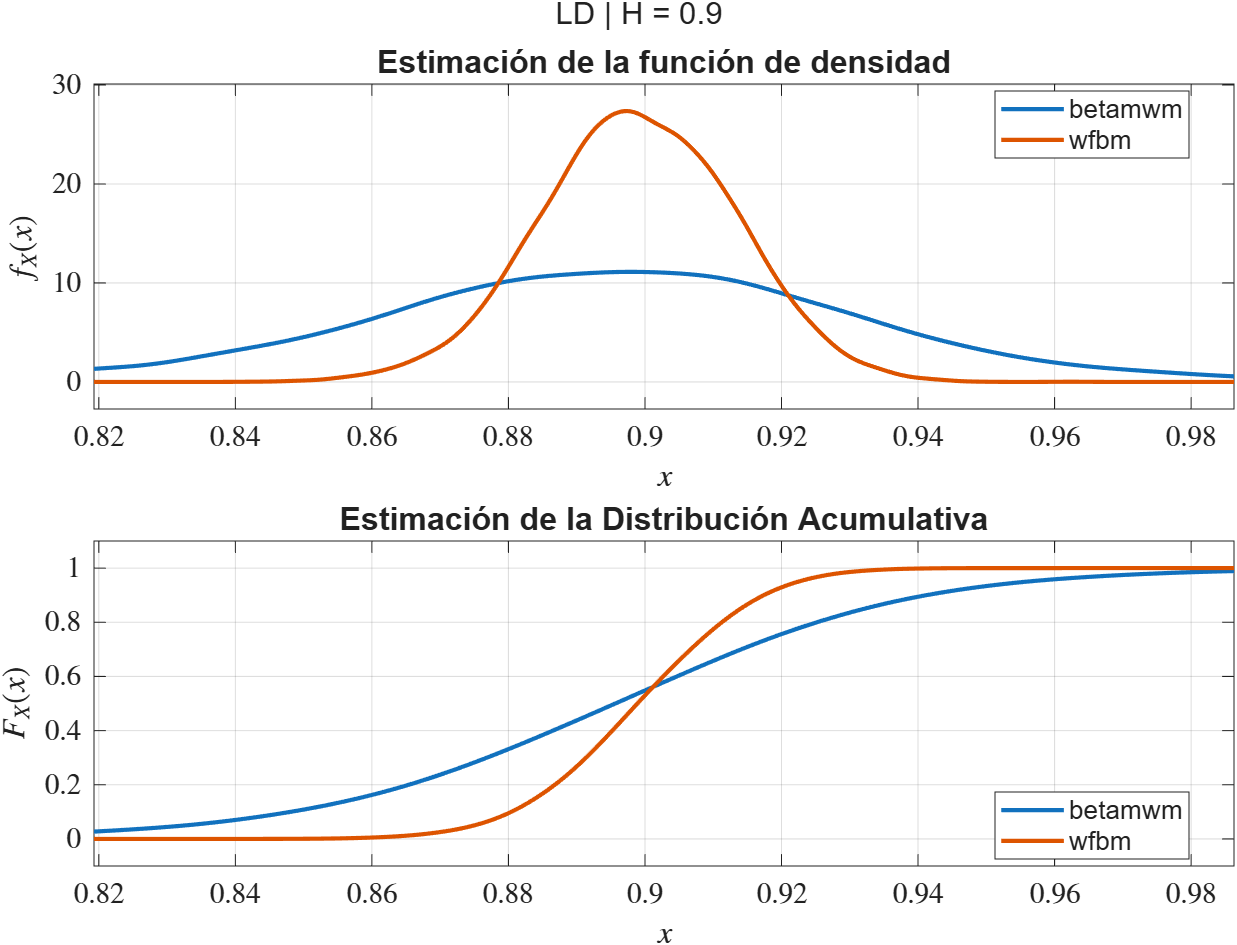
\includegraphics[width=\textwidth]{actividades/actividad2/imgs/LD_H0_9.png}
        \caption{PDF y CDF de $\hat{H}$ con LD para $H=0.9$.}
        \label{fig:ld_h09}
    \end{minipage}

\end{figure}

% ------------------------------------------------------------
\subsection{Prueba de Eficiencia}
% ------------------------------------------------------------

La eficiencia se mide comparando la varianza de $\hat{H}$ entre estimadores
para un mismo valor de $H$, esto quiere decir que el estimador con menor $\mathrm{Var}(\hat{H})$
es más eficiente. Las Figuras~\ref{fig:var_betamwm} y~\ref{fig:var_wfbm}
muestran $\mathrm{Var}(\hat{H})$ en función de $H$ real para cada combinación 
generador frente al estimador.

\begin{figure}[H]
    \centering
    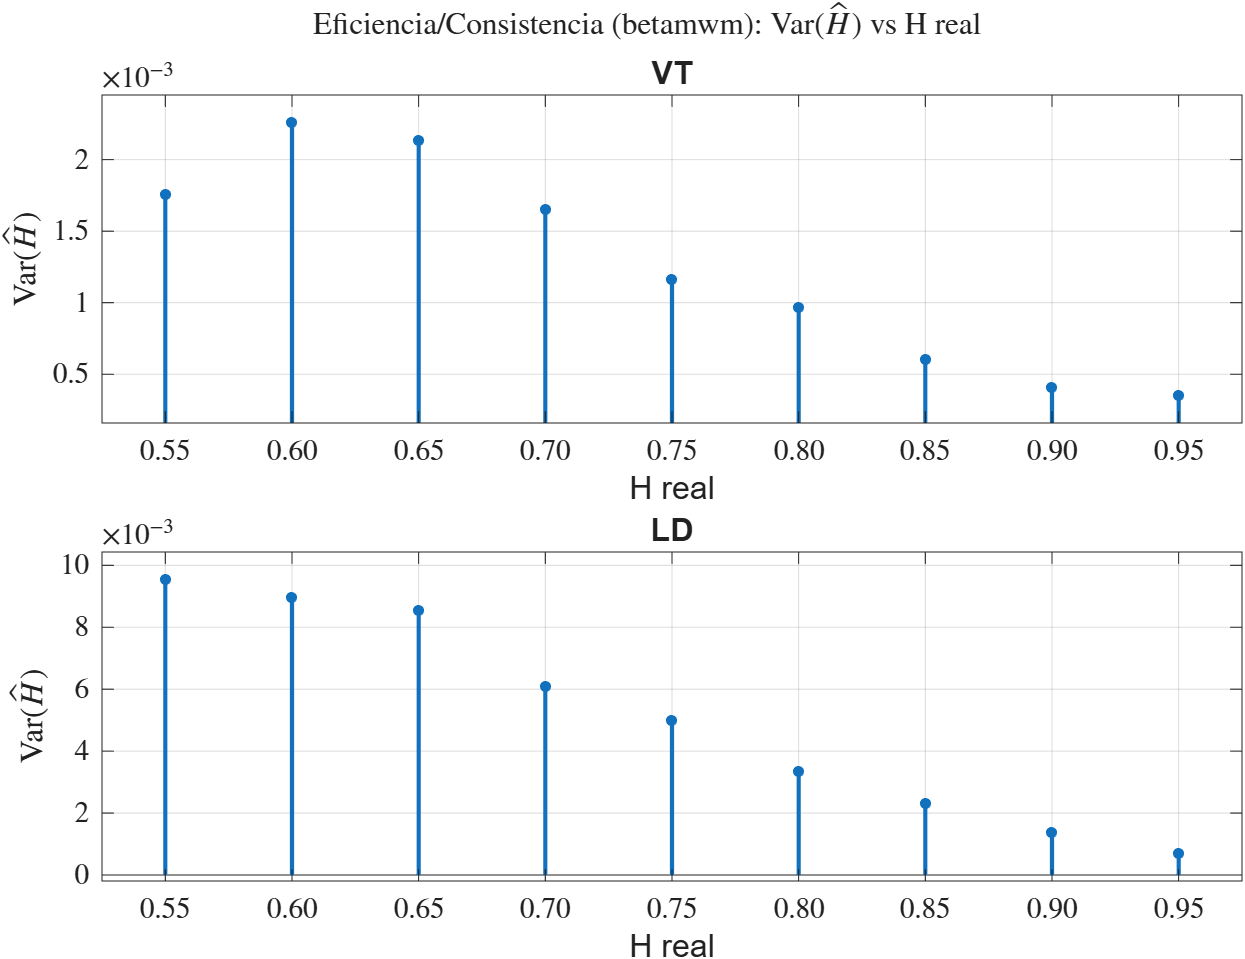
\includegraphics[width=0.75\textwidth]{actividades/actividad2/imgs/betamwm_var.png}
    \caption{Varianza de $\hat{H}$ vs.\ $H$ real para \texttt{betamwm}.
             VT (arriba) presenta varianzas del orden $10^{-3}$; LD (abajo)
             del mismo orden pero con mayor magnitud en todo el rango de $H$.}
    \label{fig:var_betamwm}
\end{figure}

\begin{figure}[H]
    \centering
    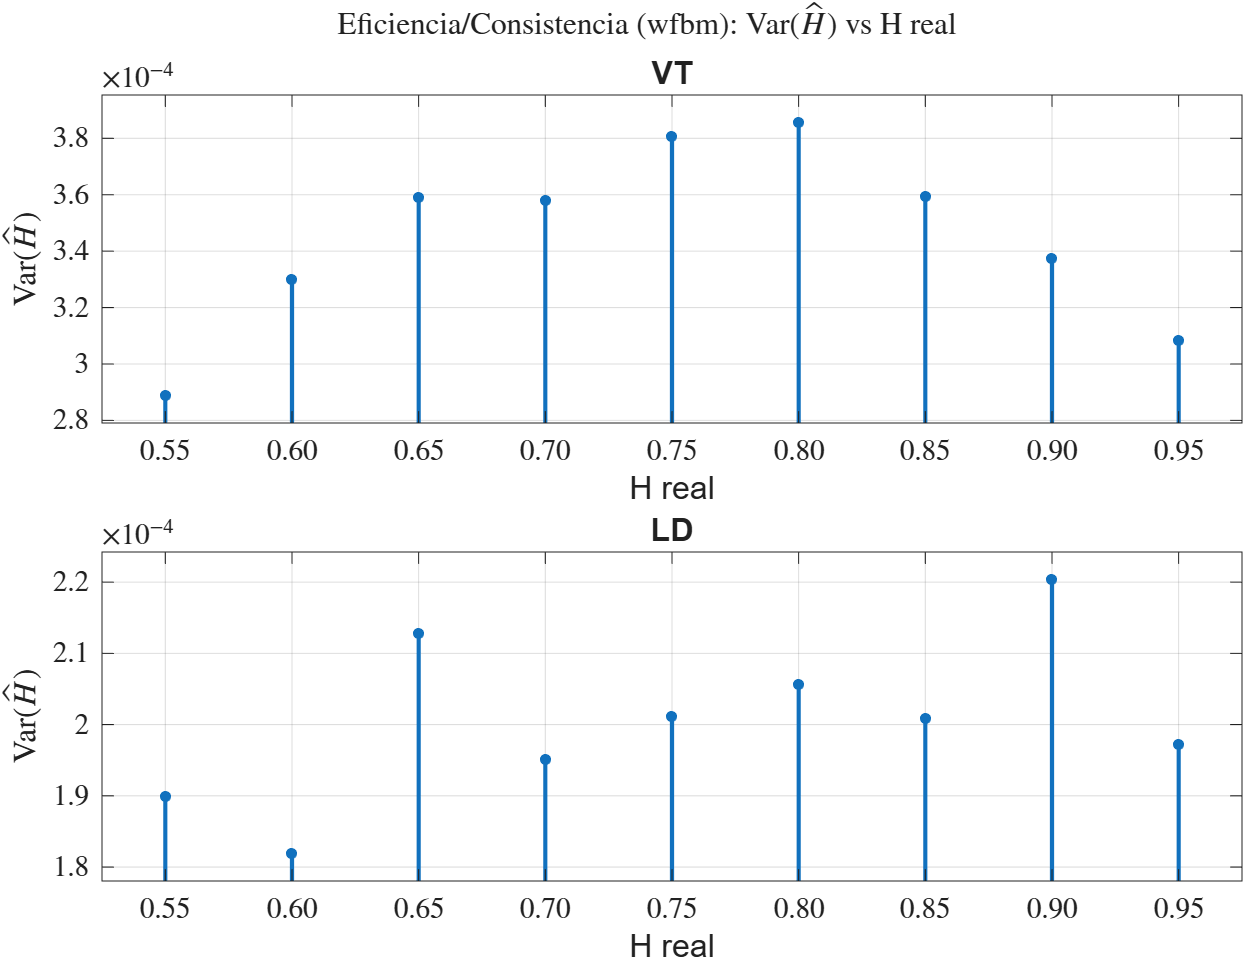
\includegraphics[width=0.75\textwidth]{actividades/actividad2/imgs/wfbm_var.png}
    \caption{Varianza de $\hat{H}$ vs.\ $H$ real para \texttt{wfbm}.
             VT (arriba) muestra varianzas del orden $10^{-4}$; LD (abajo)
             mantiene varianza menor y más estable en todo el rango.}
    \label{fig:var_wfbm}
\end{figure}

\textbf{\texttt{betamwm} (Figura~\ref{fig:var_betamwm}).} \textbf{VT es más eficiente
que LD en todo el rango de $H$}: su varianza se mantiene por debajo de
$2.25\times10^{-3}$, mientras que la de LD supera los $9\times10^{-3}$ para
$H$ bajo.

\textbf{\texttt{wfbm} (Figura~\ref{fig:var_wfbm}).} \textbf{LD es más eficiente en todo el rango}: la varianza presentada es estable alrededor de
$2\times10^{-4}$, mientras que VT fluctúa entre $2.9\times10^{-4}$ y
$3.85\times10^{-4}$.



% ------------------------------------------------------------
\subsection{Prueba de Consistencia}
% ------------------------------------------------------------

La consistencia se evalúa fijando $H$ y aumentando el tamaño de muestra
$N \in \{2^{10},\, 2^{12},\, 2^{14},\, 2^{16}\}$: un estimador consistente
debe mostrar $\mathrm{Var}(\hat{H}) \to 0$ al crecer $N$, para todo valor
de $H$ en el intervalo evaluado. Lo cual se refleja en las Figuras~\ref{fig:cons_vt} y~\ref{fig:cons_ld} por la tendencia decreciente de las curvas, además es contrastado en la Tabla~\ref{tab:consistencia_estimadores}.

\begin{figure}[H]
    \centering
    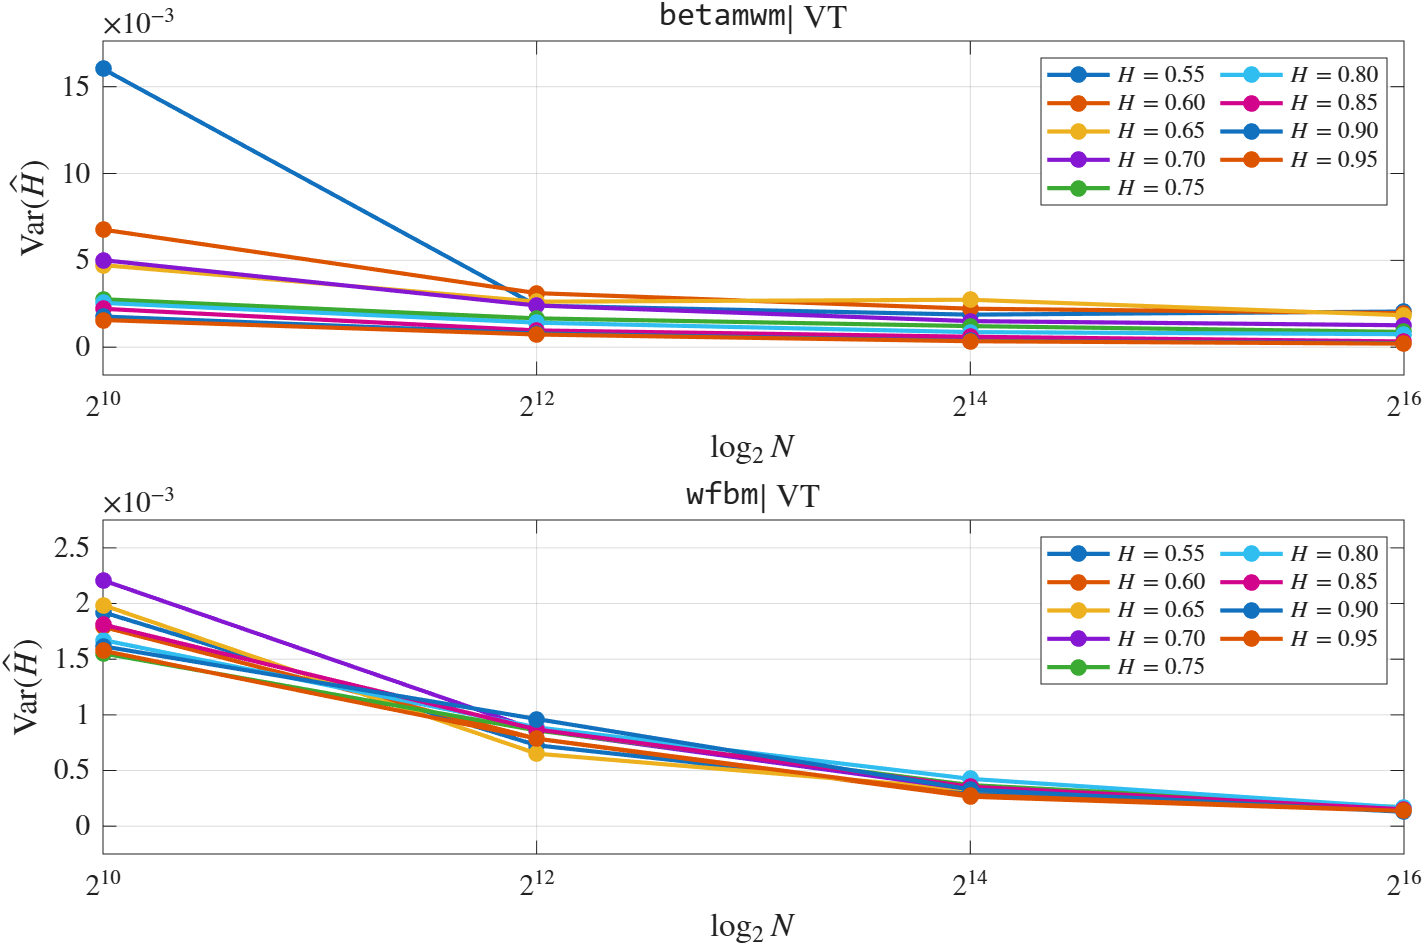
\includegraphics[width=0.95\textwidth]{actividades/actividad2/imgs/cons_VT.png}
    \caption{Consistencia del estimador VT: $\mathrm{Var}(\hat{H})$ vs.\
             $N$ para \texttt{betamwm} (arriba) y \texttt{wfbm} (abajo),
             con $H \in [0.55,\, 0.95]$ ($300$ repeticiones por punto).}
    \label{fig:cons_vt}
\end{figure}

\begin{figure}[H]
    \centering
    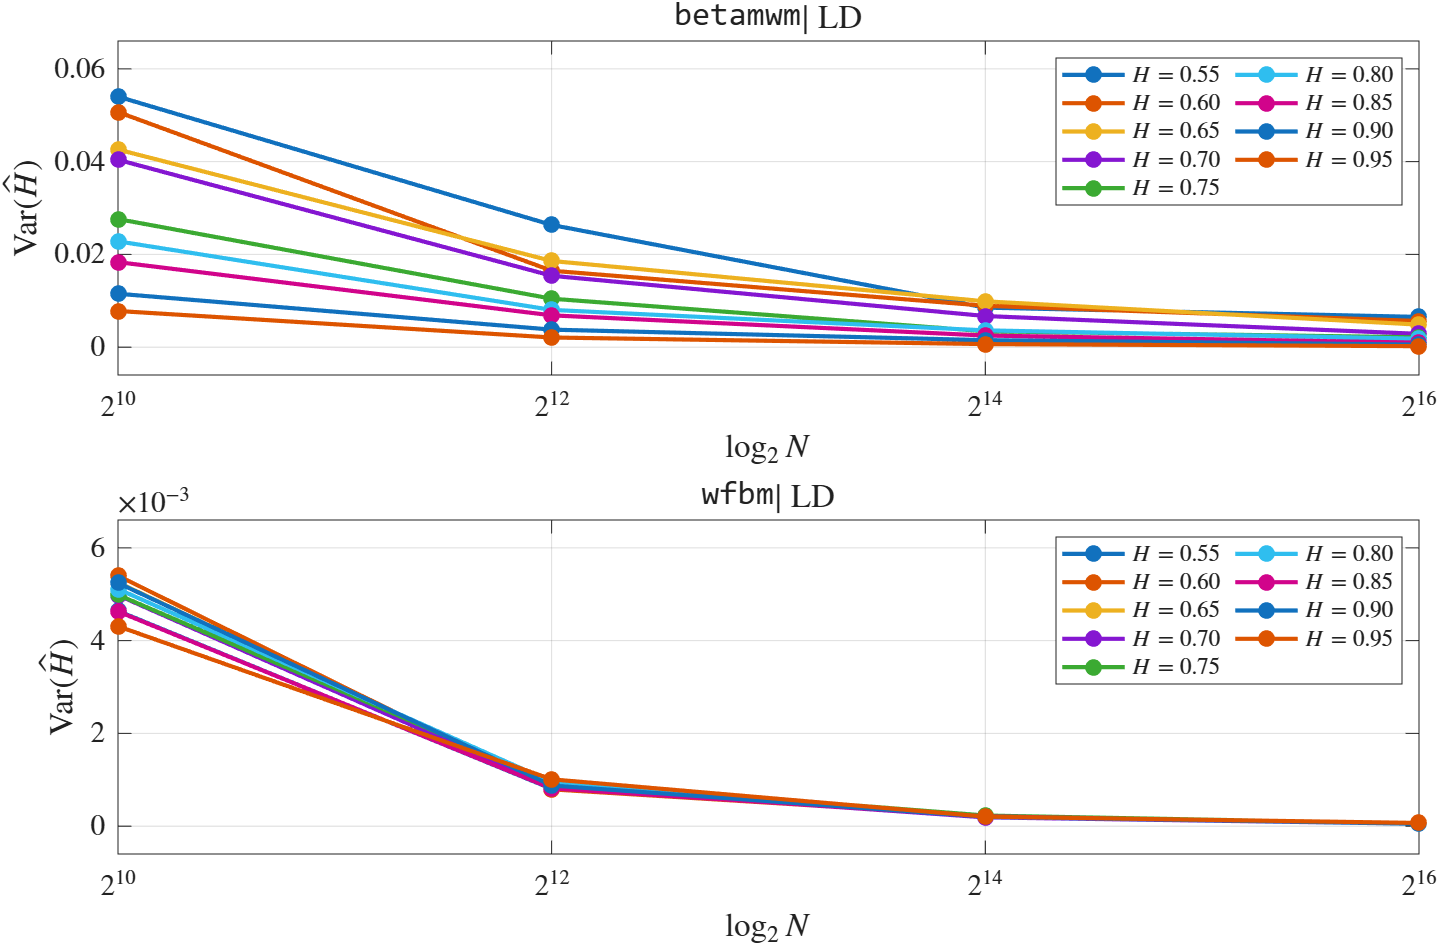
\includegraphics[width=0.95\textwidth]{actividades/actividad2/imgs/cons_LD.png}
    \caption{Consistencia del estimador LD: $\mathrm{Var}(\hat{H})$ vs.\
             $N$ para \texttt{betamwm} (arriba) y \texttt{wfbm} (abajo),
             con $H \in [0.55,\, 0.95]$ ($300$ repeticiones por punto).}
    \label{fig:cons_ld}
\end{figure}

\begin{table}[H]
\centering
\caption{Consistencia y convergencia de VT y LD sobre \texttt{betamwm} y \texttt{wfbm}.}
\label{tab:consistencia_estimadores}
\renewcommand{\arraystretch}{1.35}
\begin{tabular}{|p{3cm}|p{2cm}|p{6.8cm}|p{2.5cm}|}
\hline
\textbf{Estimador} & \textbf{Proceso} & \textbf{Comportamiento observado} & \textbf{Consistencia} \\
\hline

VT & \texttt{betamwm} &
Para $H=0.55$, la varianza cae de $1.60\times10^{-2}$ a
$2.39\times10^{-3}$, pero luego se estabiliza alrededor de
$2\times10^{-3}$ sin seguir decreciendo. Para $H\geq0.70$
la reducción es monótona, aunque lenta.
&
No consistente para $H$ bajo
\\
\hline

VT & \texttt{wfbm} &
Las curvas decrecen de forma ordenada y monótona desde
$\approx 2\times10^{-3}$ hasta $\approx 1.5\times10^{-4}$,
sin excepciones en el rango evaluado.
&
Consistente
\\
\hline

LD & \texttt{betamwm} &
La varianza decrece en todos los casos, aunque con magnitudes
mayores que VT. Para $H=0.55$ pasa de $5.40\times10^{-2}$
a $6.52\times10^{-3}$ en $N=2^{16}$.
&
Consistente, convergencia lenta
\\
\hline

LD & \texttt{wfbm} &
Las curvas se superponen casi perfectamente y descienden desde
$\approx 5\times10^{-3}$ hasta $\approx 5\times10^{-5}$,
mostrando reducción de dos órdenes de magnitud.
&
Altamente consistente
\\
\hline

\end{tabular}
\end{table}

\vspace{0.3cm}

\noindent


% ------------------------------------------------------------
\subsection{Análisis de la Actividad 2}
% ------------------------------------------------------------

\begin{table}[H]
\centering
\caption{Comparación de estimadores VT y LD por propiedad y generador.}
\label{tab:resumen_a2}
\renewcommand{\arraystretch}{1.3}
\begin{tabular}{llccc}
\toprule
\textbf{Propiedad} & \textbf{Generador} & \textbf{VT} & \textbf{LD} &
\textbf{Ganador} \\
\midrule
Sesgo & \texttt{betamwm} & Hasta $-0.071$ & Hasta $-0.005$ & \textbf{LD} \\
Sesgo & \texttt{wfbm}    & Hasta $-0.009$ & Hasta $-0.001$ & \textbf{LD} \\
\midrule
Eficiencia & \texttt{betamwm} & $\hat{\sigma}^2$ menor & $\hat{\sigma}^2$ mayor & \textbf{VT} \\
Eficiencia & \texttt{wfbm}    & $\hat{\sigma}^2$ mayor & $\hat{\sigma}^2$ menor & \textbf{LD} \\
\midrule
Consistencia & \texttt{betamwm} & Inconsistente ($H$ bajo) & Consistente, lenta & \textbf{LD} \\
Consistencia & \texttt{wfbm}    & Consistente             & Altamente consistente & \textbf{LD} \\
\bottomrule
\end{tabular}
\end{table}

